
\appendix
\section{From cartesian to Delaunay and computation of 
  $\pa_G\Delta H_\ccirc$}\label{sec:RotatingToDelaunay}
In this appendix we explain an easy way to obtain the rotating Delaunay coordinates 
from rotating cartesian (or polar) coordinates in the circular problem. First recall that $G$ can be computed  as
\[
G=r\left(-p_x\sin\phi+p_y\cos\phi\right).
\]
In a fixed level of energy $J$, knowing $G$ one can obtain $L$. Recall that
\[
J=-\frac{1}{2L^2}-G+\mu\Delta H_\ccirc
\]
The term $\mu\Delta H_\ccirc$ in cartesian only depends on $x$ and $y$, and 
can be easily computed. Then, one can use this equation to obtain $L$. 
Knowing $L$ and $G$ we can obtain the eccentricity $e$ by
\[
e=\sqrt{1-\frac{G^2}{L^2}}.
\]
Using that $r=L^2(1-e\cos u)$, one can obtain $u$ and from here $\ell$ using 
the formula $u-e\sin u=\ell$. On the other hand, from $u$ we can obtain $v$ using
\[
\tan\frac{v}{2}=\sqrt{\frac{1+e}{1-e}}\tan\frac{u}{2}.
\]
Finally, we can deduce $g$ using that $\phi=v+g$.

We devote the rest of the section to compute $\pa_G\Delta H_{\ccirc}$. Let us define
\[
N(r,v,g)=\frac{1}{\left(r^2+1-2r\cos (v+g)\right)^{1/2}}.
\]
Then,
\[
\Delta H_{\ccirc}(L,\ell,G,g)=-\frac{1-\mu}{\mu} N\left(-\frac{r(L,\ell,G)}{\mu},v(L,\ell,G),g\right)-\frac{\mu}{1-\mu} N
\left(\frac{r(L,\ell,G)}{1-\mu},v(L,\ell,G),g\right)+\frac{1}{r(L,\ell,G)}.
\]
Therefore
\[
\begin{split}
  \pa_G\Delta H_{\ccirc}(L,\ell,G,g)=&-\Bigg[-\frac{1-\mu}{\mu^2} \pa_r N\left(-\frac{r(L,\ell,G)}{\mu},v(L,\ell,G),g\right)\\
  &\qquad+\frac{\mu}{(1-\mu)^2} \pa_r N\left(\frac{r(L,\ell,G)}{1-\mu},v(L,\ell,G),g\right)\Bigg]\pa_G r(L,\ell,G)\\
  &-\Bigg[\frac{1-\mu}{\mu} \pa_v N\left(-\frac{r(L,\ell,G)}{\mu},v(L,\ell,G),g\right)\\&\qquad+\frac{\mu}{1-\mu} \pa_vN
  \left(\frac{r(L,\ell,G)}{1-\mu},v(L,\ell,G),g\right)\Bigg]\pa_G v(L,\ell,G)\\
  &-\frac{1}{r^2}\pa_G r(L,\ell,G).
\end{split}
\]
In only remains to compute $\pa_G r$ and $\pa_G v$. First, let us point out that
\[
\pa_G e=-\frac{G}{eL^2}=\frac{e^2-1}{eG}.
\]
On the other hand, using that $\ell=u-e\sin u$, one has that
\[
\pa_e u=\frac{\sin u}{1-e\cos u}.
\]
Then, since $r(L,e,\ell)=L^2(1-e\cos u(e,\ell))$,  using that
\begin{equation}\label{eq:FromUtoV}
  \cos v=\frac{\cos u -e}{1-e\cos u},
\end{equation}
we have that
\[
\pa_e r(L,e,\ell)=L^2\cos v
\]
and therefore,
\[
\pa_G r(L,\ell,G)=-\frac{G\cos v}{e}.
\]
To compute $\pa_G v$ let us point out that $\pa_G v=\pa_e v\pa_G e$. 
Therefore it only remains to compute $\pa_e v$, we obtain it using 
formula \eqref{eq:FromUtoV} and
\[
\sin v=\frac{\sqrt{1-e^2}\sin u}{1-e\cos u}.
\]
Then,
\[
\pa_e v=\frac{\sin v}{1-e^2}\left(2+e\cos v\right).
\]
and therefore,
\[
\pa_G v=-\frac{\sin v}{eG}\left(2+e\cos v\right).
\]

\section{Numerical study of the normally hyperbolic invariant manifold of the circular problem. }\label{app:NHIMCircular}

We devote this appendix to the numerical study of the hyperbolic
invariant manifold of the circular problem given in Corollary
\ref{coro:NHIMCircular} and its invariant manifolds. In other words,
we show numerical results which justify the properties of the circular
problem stated in Theorem \ref{th:NHIMCircular}.

It is well known that in numerical analysis there are several sources
of error, such as round-off errors in computer arithmetic, and
approximations of ideal mathematical objects (e.g. linear
approximation of local stable/unstable manifolds). 
In our analysis, we will try to evaluate such errors whenever
possible, and check that they are appropriately small.
We do \emph{not} claim however to give a fully rigorous proof of
Theorem~\ref{th:NHIMCircular}, which would probably require
Computer-Assisted techniques as in [Zgliczynski-Capinski],[...].

Let us make a few comments on the general strategy of our numerical
analysis. As mentioned in Section~\ref{Section:Circular}, the circular
 problem has a conserved quantity which corresponds to
energy $H$ when the system is expressed in rotating coordinates. 
Thus it is natural to fix the energy $H=h$ and perform our analysis for a given
energy $h$. This allows us to reduce the dimension of the computations by
one. Finally, we let $H$ vary and repeat the computations for all $H$
in the range of interest $H\in[H_-,H_+]$.

Another important comment is on the choice of coordinates.
For numerics we prefer Cartesian coordinates, since the equations of
motion are explicit in these coordinates.
Thus we carry out our computations of the hyperbolic structure of the
circular problem in Cartesian (section~\ref{app:NHIMCircular}).

On the other hand, for perturbative analysis we have used Delaunay
coordinates throughout this paper.
Thus, in section~\ref{sec:geometric_structure_delaunay} we explain how
to change coordinates from Cartesian to Delaunay, and 
we carry out our computations of the inner and outer maps of the
circular and elliptic problems in Delaunay
(section~\ref{sec:NumericalStudyInnerOuter}).

Regarding the integration method, we use a variable-order Taylor method
specially generated to integrate the equations of motion and
variational equations of the circular problem.
The Taylor method has been generated using the ``taylor'' package of
\`{A}.~Jorba and M.~Zou
(see~\url{http://www.maia.ub.es/~angel/taylor/}).
The main advantage of using a Taylor method is that it is very fast
for long-time integrations (without sacrificing accuracy).

\subsection{Computation of the periodic
orbits}\label{sec:computation_periodic_orbits}
Consider the circular problem in rotating cartesian coordinates
\begin{equation}\label{eq:RTBP:RotCartesian}
  H(x,y,p_x,p_y)=\frac{1}{2}(p_x^2+p_y^2)+yp_x-xp_y-\frac{1-\mu}{r_1}-\frac{\mu}{r_2},
\end{equation}
where 
\begin{align*}
r_1^2 &= (x-\mu_2)^2 + y^2, \\
r_2^2 &= (x+\mu_1)^2 + y^2.
\end{align*}

We follow the convention to place the large mass (Sun) to the left of
the origin, and the small mass (Jupiter) to the right.
(This is opposite to the astrodynamics convention).
Thus we choose $\mu_1=\mu$ as the small mass, and $\mu_2=1-\mu$ as the
large mass.
Notice that equation~\eqref{eq:RTBP:RotCartesian} is reversible with
respect to the involution 
\begin{equation} \label{involutionCartesian}
R(x,p_x,y,p_y) = (x,-p_x,-y,p_y).
\end{equation}
Thus, a solution of the system is symmetric if and only if it
intersects the symmetry axis $\mathrm{Fix}(R) = \{y=0,\ p_x=0\}$.
This symmetry will facilitate our numerical computations. Note that the involution $R$ is just the involution \eqref{def:involution} expressed in rotating cartesian coordinates.

Let the energy be fixed to $H=h$. 
We look for a resonant periodic orbit $\gamma_h$
of~\eqref{eq:RTBP:RotCartesian} in the level of energy $h$.
As a first approximation to $\gamma_h$, we look for a resonant
periodic orbit of the two-body problem, i.e. of the
Hamiltonian~\eqref{def:HamDelaunayCirc} with $\mu=0$.
Let us denote the approximate periodic orbit by
$\tilde \gamma_h=(L,\ell,G,g)$. 
The actions $L$ and $G$ are determined by the resonant condition
$L^3=7$ and energy condition $-\frac{1}{2L^2}-G=h$. 
To determine $\tilde \gamma_h$ completely, we choose that the
Asteroid is initially at the perihelion, i.e. we impose an initial
condition $\tilde \gamma_h(t=0)=(L^0,\ell^0,G^0,g^0)$ with mean anomaly
$\ell^0=0$ and argument of perihelion $g^0=0$.
Switching to cartesian coordinates, we obtain an initial condition
$(x^0,p_x^0,y^0,p_y^0)$ with $p_x^0=0$ and $y^0=0$.

Next we refine the trajectory $\tilde \gamma_h$ into a true periodic
orbit $\gamma_h$ for the system~\eqref{eq:RTBP:RotCartesian} with
$\mu=\mu_J$.
Consider the Poincar\'e section
\[ \Sigma^+ = \{ y=0,\ p_y>0 \} \]
in the circular problem~\eqref{eq:RTBP:RotCartesian}, and let $P\colon\
\Sigma^+\to\Sigma^+$ be the associated Poincar\' e map. Since we are in rotating coordinates, this section corresponds to collinear configurations
of the three bodies.

\begin{remark}
In numerical integrations, we use a variable-order Taylor method with
local error tolerance $10^{-16}$.
Moreover, a point is considered to be on the Poincar\'e section whenever
$|y|<10^{-16}$ and $p_y>0$.
\end{remark}
Furthermore, the momentum variable $p_y$ can be eliminated. 
Assuming that $\partial_{p_y} H \neq 0$, it can be recovered from the
other variables using the energy condition $H(x,p_x,y,p_y)=h$. 
Hence, the Poincar\'e map is a two-dimensional symplectic map
at each energy level, acting only on $(x,p_x)$.

Notice that, in the rotating frame, a 7:1 resonant periodic orbit
makes $6$ turns around the origin. See Figure~\ref{fig:trtbp}.
In principle, we could look for the periodic orbit as a periodic point
$p=(x,p_x)$ of the Poincar\'e map: $p=P^6(p)$. This would imply solving
a system of two equations.
Thanks to the reversibility~\eqref{involutionCartesian},
in fact it is only necessary to solve one equation.
Notice that our initial condition $(x,p_x)$ is at the symmetry
section $\{y=0,\ p_x=0\}$, so the periodic orbit must be symmetric. 
Thus it is enough to impose the condition that the trajectory
$\gamma_h(t)$ after \emph{half} the period is again at the symmetry
section. 
Hence we set up the problem as simple one-dimensional root finding:
we look for a point $p=(x,0)$, such that its third iterate $P^3(p)$
has momentum $p_x=0$:
\[ \pi_{p_x}(P^3(p)) = 0. \]
(Here, $\pi_{p_x}\colon \RR^2\to \RR$ is the projection onto the $p_x$
component).

In order to solve this problem, we use a a Newton-like method. 
Specifically, we use a modified version of Powell's Hybrid method (see
the GSL manual for details) without scaling.
In our computations, the Newton method converges in less than 5
iterations.
As a test of the software, we have checked that the rate of
convergence of the Newton method is quadratic.

\begin{remark}
We ask for an accuracy of $10^{-14}$ in the Newton method,
i.e. a point $p=(x,0)$ is accepted as a root if and only if its third iterate
$P^3(p)$ has momentum $|p_x|<10^{-14}$.
\end{remark}

For the Newton method, we need to compute the derivative of the Poincar\'e map.
For each $\xi\in \RR^4$, let $u(t,\xi)$ be the solution of the system with
initial condition $u(0,\xi)=\xi$.
Let $T:\Sigma^+\to \RR$ be the Poincar\'e return time.
The derivative of the Poincar\'e map at a point $p\in \RR^4$ is given by
the partial derivative $DP(p)=u_\xi(T(p),p)$.
It is well-known that $u_\xi(t,p)$ is the matrix solution of the
variational equation
\[ \dot W = Df(u(t,p))W, \]
where $f$ is the vectorfield of the circular problem.
We compute $DP(p)$ by numerically integrating the variational
equation using the Taylor method mentioned above. 

\begin{figure}{}
\psfrag{x}{$x$}
\psfrag{y}{$y$}
\psfrag{z}{$p$}
\psfrag{P1}{$P(p)$}
\psfrag{P2}{$P^2(p)$}
\psfrag{P3}{$P^3(p)$}
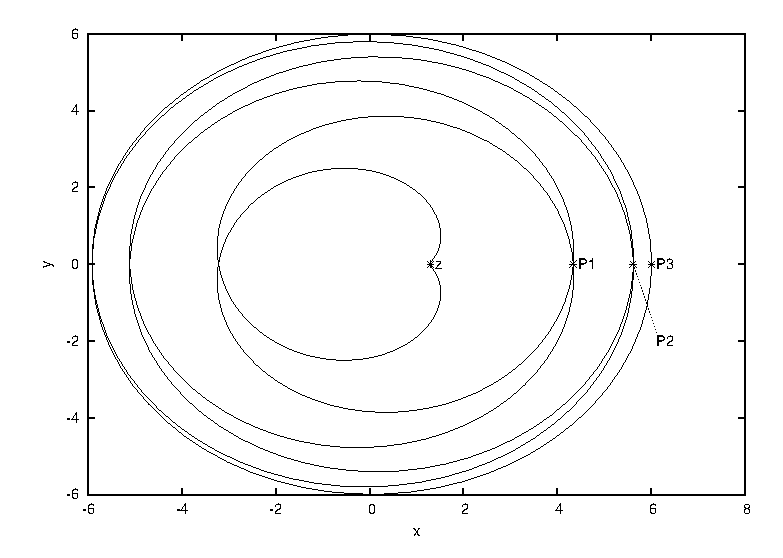
\includegraphics{figs/trtbp}
\caption{Resonant periodic orbit $\gamma_{-1.6}$ of the circular
problem in rotating cartesian coordinates.}
\label{fig:trtbp}
\end{figure}

For illustration, let us show some numerical results corresponding to
the energy value $H=-1.6$.
The first approximation $\tilde \gamma_{-1.6}$ from the two-body
problem has initial condition $p^0=(x^0,p_x^0)=(1.30253\cdots,0)$.
After refining this initial condition via the Newton method, we obtain
a resonant periodic orbit $\gamma_{-1.6}$ of the circular problem passing
through the point $p=(x,p_x)=(1.29858\cdots,0)$, with period
$T_{-1.6}=44.01796\cdots \sim 14\pi$. See Figure~\ref{fig:trtbp}. 
The periodic orbit $\gamma_{-1.6}$ is symmetric, with the points $p$
and $P^3(p)$ located at the symmetry section (they have $y=0$ and $p_x=0$).
Notice that, in rotating coordinates, the trajectory of the Asteroid
makes 6 turns around the origin before closing up at the point $p$.

\begin{figure}
\psfrag{H}{$H$}
\psfrag{T}{$T_H - 14\pi$}
\psfrag{T2XXXXXXX}{$T_H - 14\pi$}
\psfrag{L2XXXXXXX}{$L_{\max}$}
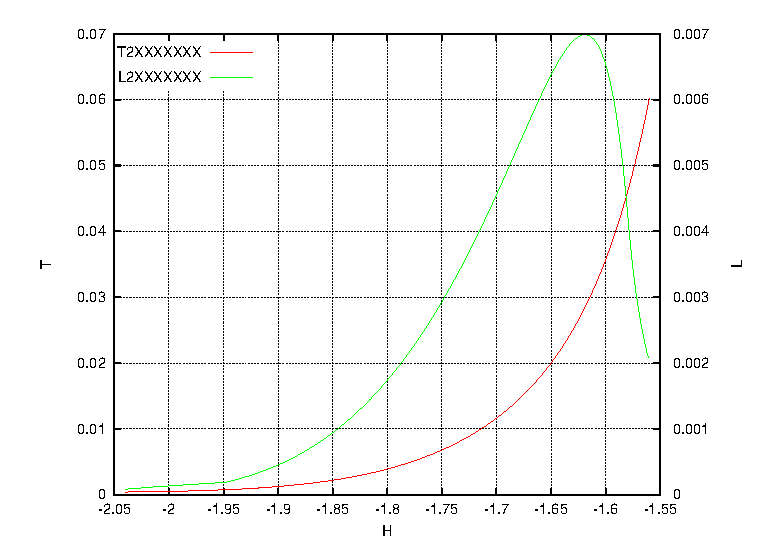
\includegraphics{figs/porbits}
\caption{Resonant family of periodic orbits.
We show normalized period $T_H - 14\pi$, and maximum deviation of $L$
component with respect to the resonant value $7^{1/3}$ (see
equation~\eqref{eq:Ldeviation}).}
\label{fig:porbits}
\end{figure}

Finally, we let $H$ change and, using this procedure, we are able to
obtain the resonant periodic orbit for energy levels 
\[ H \in [\bar H_-, \bar H_+] = [-2.04,-1.56]. \] 
See Figure~\ref{fig:porbits}.
This family of resonant periodic orbits constitutes the normally
hyperbolic invariant manifold $\Lambda_0$ given in
Corollary~\ref{coro:NHIMCircular}. 
Notice that the period $T_H$ stays close to the resonant period $14\pi$ of the unperturbed system.
From Figure~\ref{fig:porbits}, we obtain the bound
\[ |T_H - 14\pi| < 60\mu, \]
which is the first bound given in Theorem \ref{th:NHIMCircular}.


To determine the stability of the periodic orbit $\gamma_h$, we
compute the eigenvalues $\lambda$ and $\lambda^{-1}$ of the matrix
$DP^6(p)$, where $DP^6(p)$ is the linearization of the iterated
Poincar\'e map $P^6$ about the fixed point $p$. 
(Since $DP^6(p)$ is a $2\times2$ matrix, the eigenvalues are trivial
to compute.)

\begin{figure}
\psfrag{H}{$J$}
\psfrag{lu}{$\ln(\lambda)$}
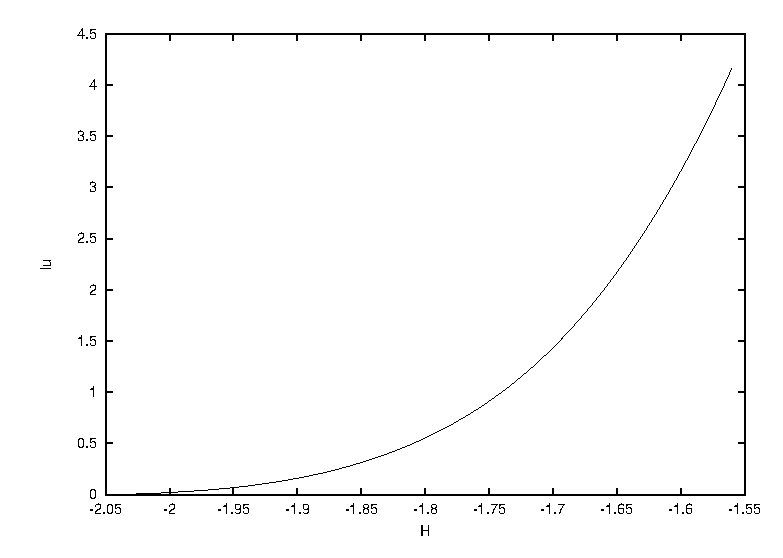
\includegraphics{figs/hypers}
\caption{Characteristic exponent $\ln(\lambda)$ as a function of
energy level $J$ (the other exponent is $-\ln(\lambda)$).}
\label{fig:hypers}
\end{figure}

Figure~\ref{fig:hypers} shows the characteristic exponents
$\ln(\lambda)$, $\ln(\lambda^{-1})$ as a function of energy.
The family of periodic orbits is strongly hyperbolic as $H \to \bar
H_+$, and weakly hyperbolic as $H\to \bar H_-$.
Note that one would expect that we are in a  nearly integrable regime
since $\mu$ is small. Then one would expect the eigenvalues to be
close to 1.
Nevertheless, in this problem the non-integrability is very noticeable
when one increases $\mu$ to $\mu=\mu_J=10^{-3}$. This is due to the effect of
the perturbing body (Jupiter) on the Asteroid, as the Asteroid passes
close to it.

Furthermore, we verify that the (square of the) semi-major axis $L$ stays
close to the resonant value $7^{1/3}$.
Integrating the periodic orbit in Delaunay coordinates
$\gamma_H(t)=(L(t),\ell(t),G(t),g(t))$ over one period $T_H$, we compute
the quantity
\begin{equation} \label{eq:Ldeviation}
 L_{\max}(H) = \max_{t \in [0,T_H)} |L_H(t)-7^{1/3}|.
\end{equation}
The function $L_{\max}(H)$ is plotted in figure~\ref{fig:porbits}.
Notice that we obtain the bound
\[ |L_H(t)-7^{1/3}| < 7\mu \]
for all $t\in \RR$, which is stated in Theorem \ref{th:NHIMCircular}.

\begin{figure}
\psfrag{x}{$x$}
\psfrag{y}{$y$}
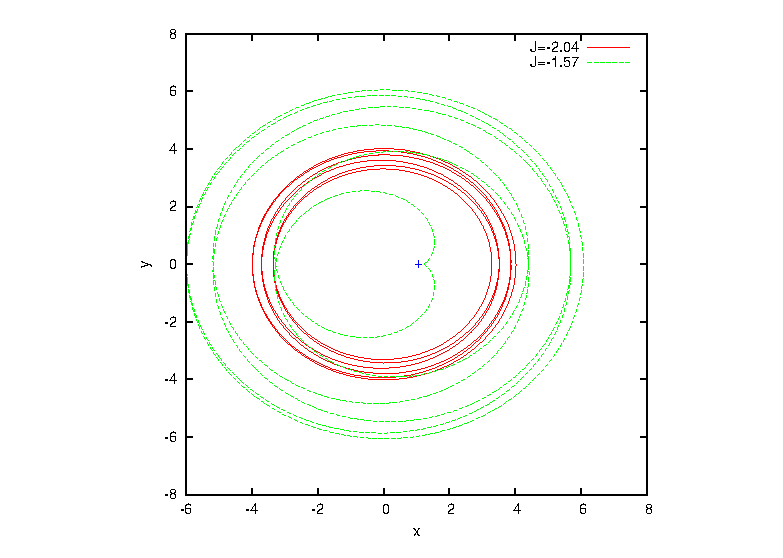
\includegraphics{figs/trtbp_porbits}
\caption{Extremal periodic orbits of the family: circular periodic
orbit with $H=\bar H_-$ (in red), elliptical periodic orbit with
$H=\bar H_+$ (in green). The Lagrange equilibrium point $L_2$ is
marked with a '+' symbol.}
\label{fig:trtbp_porbits}
\end{figure}

Let us briefly describe the family of periodic orbits $\gamma_H$. 
For illustration, see Figure~\ref{fig:trtbp_porbits}.

XXXXX PR: We should try to explain the family in terms of bifurcations
of periodic orbits. XXXXX

At one endpoint of the family, as $H \to \bar H_-$, the periodic orbit
$\gamma_H$ tends to a circular orbit of period $14\pi$ centered at the
origin and passing far away from the primaries (Sun and Jupiter).
Moreover, $\gamma_H$ looses hyperbolicity when $H \to \bar H_-$.
For instance, the periodic orbit $\tilde \gamma(\bar H_-)$ of the two-body
problem approximation has eccentricity $e(\bar H_-)=0.09989\cdots$.

At the other endpoint of the family, as $H \to \bar H_+$, the periodic
orbit $\gamma_H$ tends to a homoclinic loop of the Lagrangian
equilibrium point $L_2$ that makes $6$ turns around the Sun-Jupiter
system. 
(In rotating cartesian coordinates, $L_2$ is located on the $x$ axis at
the point $x_2 \simeq 1.068$).\ 
This explains the fact that the period $T_H$ ``explodes'' as $H \to
\bar H_+$. Since we are interested in working close to the resonance,
we avoid energies $H > \bar H_+$ where the period explodes.


\subsection{Computation of invariant manifolds}
\label{sec:invariant_manifolds}


In this section, we compute the stable and unstable invariant
manifolds associated to the periodic orbits found in the previous
section. 

Consider first a fixed energy level $H=h$.
Let $\gamma_h$ be the resonant periodic orbit of the circular problem
found in the previous section. 
To compute the invariant manifolds of the periodic orbit, we continue
using the iterated Poincar{\'e} map.
Thus we look for (one dimensional) invariant manifolds of a hyperbolic
fixed point at each energy level.  
Let $p \in \gamma_h$ be a hyperbolic fixed point of the iterated
Poincar\'e map $\sixmap = P^6$. 
Let $\lambda, \ \lambda^{-1}$ be the eigenvalues of $D\sixmap(z)$ with
$\lambda>1$, and $v_u, v_s$ be the associated eigenvectors.

Assume that we want to compute the unstable manifold $W^u(p)$.
Let $\eta$ be a small displacement in the unstable direction $v_u$.
We approximate a piece of the local manifold by the linear segment
between the points $p+\eta v_u$ and $\sixmap(p+\eta v_u)$.
We call this segment a \emph{fundamental domain}.
We discretize the fundamental domain into an array of points, and
iterate them by $\sixmap$ to globalize the manifold.
(The stable manifold is computed analogously using the inverse map
$\sixmap^{-1}$.)

The error commited in the local approximation
$ \sixmap(p+\eta v_u) = p + \lambda \eta v_u + \OO(\eta^2) $
of the manifold is given by
\[ \mathrm{err}(\eta) = \left\|\sixmap(p+\eta v_u) - p - \lambda \eta v_u \right\| \in \OO(\eta^2).
\]
%Similarly, in the stable case,
%\[ err_s(\eta) =  ||\sixmap^{-1}(z+\eta v_s)-z-\frac{1}{\rho_s}\eta v_s|| \in
%O(\eta^2). \]

\begin{remark} \label{rem:displacement}
For each energy level $H$, we choose a displacement $\eta=\eta(H)$
such that the local error is $\mathrm{err}(\eta) < 10^{-12}$.
\end{remark}

\begin{figure}
\psfrag{x}{$x$}
\psfrag{px}{$p_x$}
\psfrag{p0}{$p_0$}
\psfrag{p1}{$p_1$}
\psfrag{p2}{$p_2$}
\psfrag{p3}{$p_3$}
\psfrag{p4}{$p_4$}
\psfrag{p5}{$p_5$}
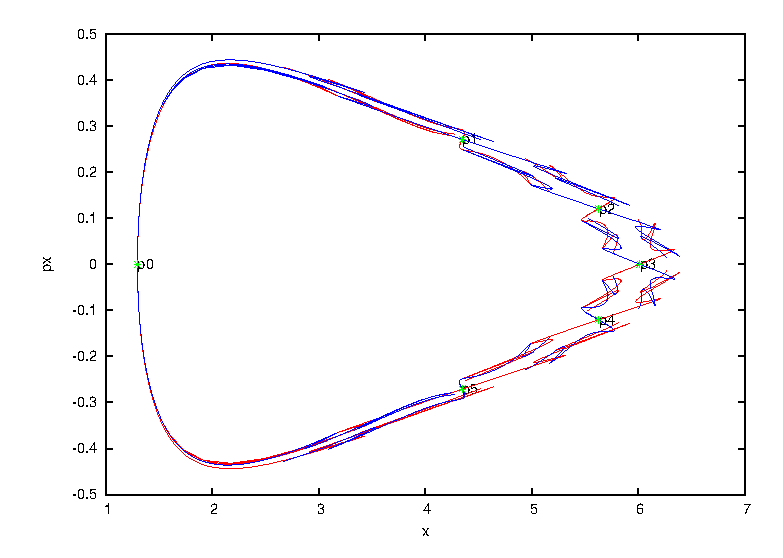
\includegraphics{figs/invmfld_it}
\caption{Invariant manifolds of the fixed points $p_0, p_1,\dots,p_5$
on the section $\Sigma^+$.
Unstable manifolds are plotted in red, stable in blue.
The fixed points are marked in green.}
\label{fig:invmfld_it}
\end{figure}

One can think of $p$ as a fixed point of the iterated Poincar\'e map
$\sixmap = P^6$, or as a $6$-periodic point of the Poincar\'e map $P$.
If $p_i = P^i(p)$ are the iterates of $p$ for $i=0,\dots,5$, then
$p_i$ are also fixed points of $\sixmap$. 
They have associated unstable and stable manifolds, which can be obtained from
$W^{u,s}(p)$ by iteration.

For illustration, let us show some numerical results corresponding to
the energy value $H=-1.6$.
Figure~\ref{fig:invmfld_it} shows the manifolds of all iterates
$\{p_i\}_{i=0,\dots,5}$.
Notice that the dynamics in Figure~\ref{fig:invmfld_it} is reversible
with respect to the symmetry section $\{y=0,\ p_x=0\}$, as discussed
in the previous section (equation~\eqref{involutionCartesian}).
Figure~\ref{fig:invmfld_it} shows that the manifolds do intersect
transversally at different homoclinic points.
We are interested in measuring the splitting angle between the
manifolds.
Unfortunately, the homoclinic points do not lie on the symmetry axis, which
would be very useful in order to compute them.

\begin{figure}
\psfrag{x}{$x$}
\psfrag{px}{$p_x$}
\psfrag{p0}{$p_0$}
\psfrag{p1}{$p_1$}
\psfrag{p2}{$p_2$}
\psfrag{p3}{$p_3$}
\psfrag{p4}{$p_4$}
\psfrag{p5}{$p_5$}
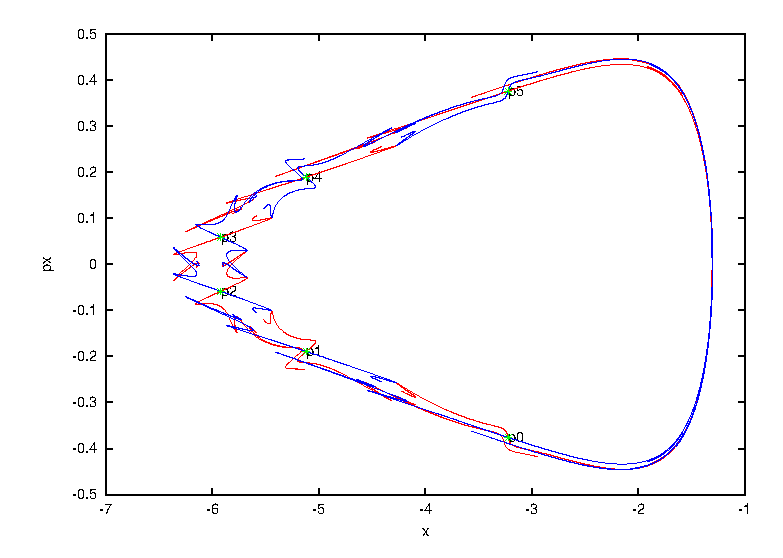
\includegraphics{figs/invmfld2}
\caption{Invariant manifolds on the section $\Sigma^-$.}
\label{fig:invmfld2}
\end{figure}

\begin{figure}
\psfrag{x}{$x$}
\psfrag{px}{$p_x$}
\psfrag{p2}{$p_2$}
\psfrag{p3}{$p_3$}
\psfrag{Wu1p3}{$W^{u,1}(p_3)$}
\psfrag{Ws2p3}{$W^{s,2}(p_3)$}
\psfrag{Ws1p2}{$W^{s,1}(p_2)$}
\psfrag{Wu2p2}{$W^{u,2}(p_2)$}
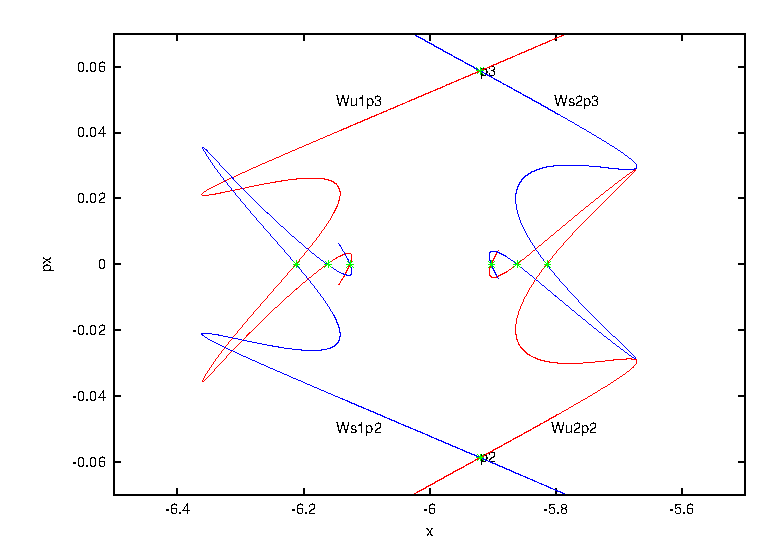
\includegraphics{figs/invmfld2_it23}
\caption{Invariant manifolds of the points $p_2$ and $p_3$ on the
section $\Sigma^-$. Due to the symmetry, points that lie on the line
$p_x=0$ (marked in green) are intersection points.}
\label{fig:invmfld2_it23}
\end{figure}


In order to have the homoclinic points lie on the symmetry axis, we
recompute the manifolds on the new Poincar\'e section
\[ \Sigma^- = \{y=0,\ p_y<0\}. \]
Numerically, we just transport points on the unstable manifold from
section $\Sigma^+$ to section $\Sigma^-$ by the forward flow, and
points in the stable manifold by the backward flow.
See Figures~\ref{fig:invmfld2} and~\ref{fig:invmfld2_it23}.
Now the points that lie on the symmetry line $p_x=0$ are homoclinic
points.


\subsection{Computation of transversal homoclinic points and splitting
angle}
\label{sec:homoclinic_points}


In this section, we compute the angle between the invariant manifolds
at one of the  transversal intersections. 
We will restrict the range of energy values to
\[ H\in[H_-,H_+]=[-1.81,-1.56], \]
or equivalently the range of eccentricities to
$ e\in[e_-,e_+]=[0.48,0.66]$.
This is the range where we can validate the accuracy of our
computations (see section~\ref{sec:accuracy_computations}).
Below $e_-=0.48$, the splitting size becomes comparable to the
numerical error that we commit in double precision arithmetic. 

\begin{remark}
In this paper we concentrate on proving the existence of global
instabilities in the Restricted three-body problem; we are not so much
concerned with finding the \emph{maximal} range of eccentricities
along which the Asteroid drifts.
Thus we do not investigate the behavior of the splitting below
$e_-$.
However, we are convinced that the maximal range of eccentricities is
larger than $[e_-,e_+]$, in particular that the lower bound can be
pushed well below $e_-$.  
We think that our mechanism of instability applies to this larger
range of eccentricities.
In fact, it is possible to study such exponentially small splitting
using more sophisticated numerical methods, such as multiple-precision
arithmetic, and high-order approximation of local invariant manifolds,
see for instance~\cite{FontichSimo1990, DelshamsRamirez1999,
GelfreichSimo2008}.
\end{remark}

\begin{figure}
\psfrag{x}{$x$}
\psfrag{px}{$p_x$}
\psfrag{p2}{$p_2$}
\psfrag{p3}{$p_3$}
\psfrag{z1}{$z_1$}
\psfrag{z2}{$z_2$}
\psfrag{Wu1p3}{$W^{u,1}(p_3)$}
\psfrag{Ws2p3}{$W^{s,2}(p_3)$}
\psfrag{Ws1p2}{$W^{s,1}(p_2)$}
\psfrag{Wu2p2}{$W^{u,2}(p_2)$}
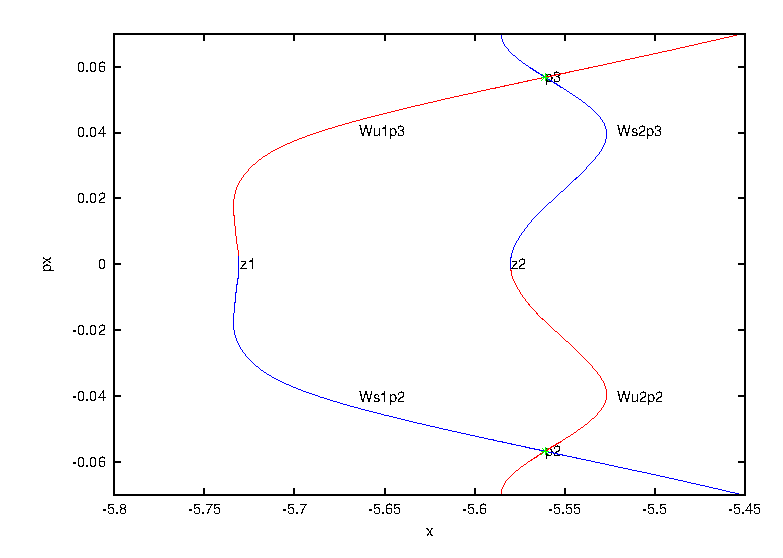
\includegraphics{figs/invmfld2_it23_H174}
\caption{Invariant manifolds of the points $p_2$ and $p_3$ for the energy
level $H=-1.74$.}
\label{fig:invmfld2_it23_H174}
\end{figure}

Consider first a fixed energy level $H=h$ that is close to the
unperturbed situation, e.g. $H=-1.74$. 
The corresponding manifolds are given in
Figure~\ref{fig:invmfld2_it23_H174}.
In general, there are uncountably many intersection points.
For instance, in Figure~\ref{fig:invmfld2_it23} we show six intersections on
the symmetry line.
However, when the perturbation is small, there is one distinguished
intersection point located ``in the middle'' of the homoclinic.
We call it the \emph{primary} intersection point.

Let us compute the primary intersection point $z_1$ corresponding to
the ``outer'' splitting of the manifolds $W^{u,1}(p_3)$ and
$W^{s,1}(p_2)$.
For $H=-1.74$, the \emph{primary} intersection $z_1$ corresponds to
the \emph{first} intersection of the manifolds with the $p_x=0$ line,
as we grow the manifolds from the fix points.
Thanks to the symmetry, it is enough to look for the intersection of
$W^{u,1}(p_3)$ with the $p_x=0$ axis, because $W^{s,1}(p_2)$ must also
intersect the axis at the same point.

To compute the intersection point $z_1$, we continue using a linear
approximation of the local manifold, and propagate a fundamental
domain in the local manifold by iteration.
Let $v_u$ be the unstable eigenvector associated to the point $p_3$.
Consider the fundamental segment $l_u$ between the points $p_3+\eta
v_u$ and $\sixmap(p_3+\eta v_u)$, as in the previous section.
First we look for the \emph{smallest} natural $n$ such that
$\sixmap^n(l_u)$ intersects the $p_x=0$ axis.
%(For our example periodic orbit $\gamma_{-1.74}$ we need $n=15$
%iterations.)
Then we use a standard numerical method (bisection-like
one-dimensional root finding) to find a point $z_u$ in the fundamental
segment $l_u$ such that
\[ \pi_{p_x}(\sixmap^{n}(z_u))=0. \]
Thus we obtain the homoclinic point $z_1 = \sixmap^{n}(z_u)$ in
Figure~\ref{fig:invmfld2_it23_H174}.
Numerically, we verify that $z_1$ is in the the $p_x=0$ axis within
$10^{-10}$ tolerance.

\begin{figure}
\psfrag{H}{$H$}
\psfrag{x}{$x$}
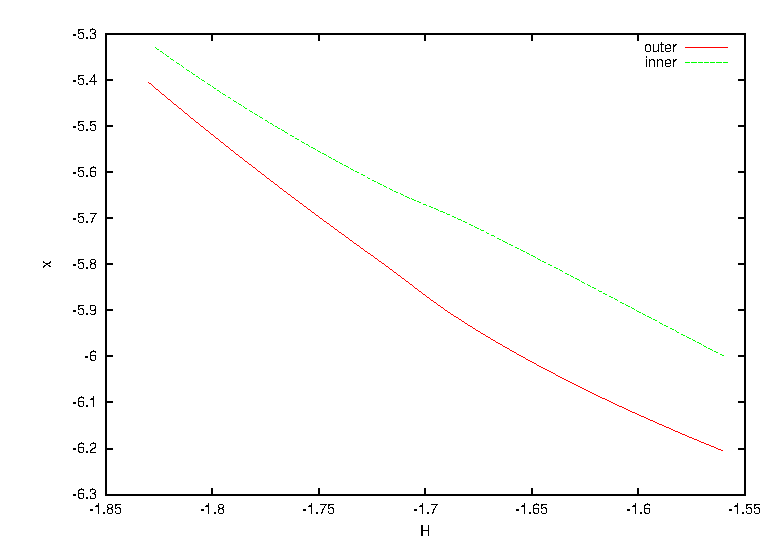
\includegraphics{figs/intersec}
\caption{Family of primary intersection points corresponding to outer
and inner splitting. 
For every energy level $H$, we plot the $x$ coordinate of the
intersection point $z_1$ and $z_2$ (the $p_x$ coordinate is equal to
zero). Notice that both families are continuous.}
\label{fig:intersec}
\end{figure}

Finally, we vary energy $H$ and use a continuation method to obtain
the family of primary intersections $\{z_1\}_H$, using as seed the
primary intersection $z_1(H=-1.74)$ found above.
See Figure~\ref{fig:intersec}.

\begin{remark}
For low energy levels (such as $H=-1.74$), corresponding to weak
hyperbolicity, the invariant manifolds behave as if they were close to
integrable, and the primary intersection corresponds to the
\emph{first} intersection of the manifolds with the $p_x=0$ axis.
For high energy levels (such as $H=-1.6$), corresponding to strong
hyperbolicity, the manifolds develop some folds, and thus the primary
intersection may not correspond to the \emph{first} intersection of
the manifolds with the $p_x=0$ axis. See
Figure~\ref{fig:invmfld2_it23}.

In practice, we first identify the primary intersection at low energy
levels, and then use a continuation method to obtain. the primary
family of intersections up to high energy levels.
\end{remark}

Analogously, we compute the family of primary intersections
$\{z_2\}_H$ corresponding to the inner splitting.
See Figure~\ref{fig:intersec}.

Let us now compute the splitting angle between the manifolds $W^{u,1}(p_3)$
and $W^{s,1}(p_2)$ at the point $z_1$.
For illustration, we show some numerical results corresponding
to the energy value $H=-1.74$.
First we need the tangent vectors $w_u$ and $w_s$ to the manifolds at
$z_1$. See Figure~\ref{fig:splitangle}.
As found above, let $z_u$ be the point in the unstable fundamental
segment that maps to $z_1$, i.e. $\sixmap^{n}(z_u) = z_1$.
Consider the tangent vector $v_u$ to the manifold $W^{u,1}(p_3)$ at
the point $z_u$. 
(Recall that at this point the linear approximation is good enough, so
we can use as $v_u$ the unstable eigenvector.)
Multiply $v_u$ by the Jacobian of $\sixmap$ at the successive iterates
$\sixmap^{i}(p_u)$, for $i=0,...,n-1$.
This way, we obtain the tangent vector to the unstable manifold at
$z_1$. Let us denote this vector $w_u=(w_1,w_2)$.
We normalize it to $||w_u||=1$.

\begin{figure}
\psfrag{x}{$x$}
\psfrag{px}{$p_x$}
\psfrag{z}{$z_1$}
\psfrag{wu}{$w_u$}
\psfrag{ws}{$w_s$}
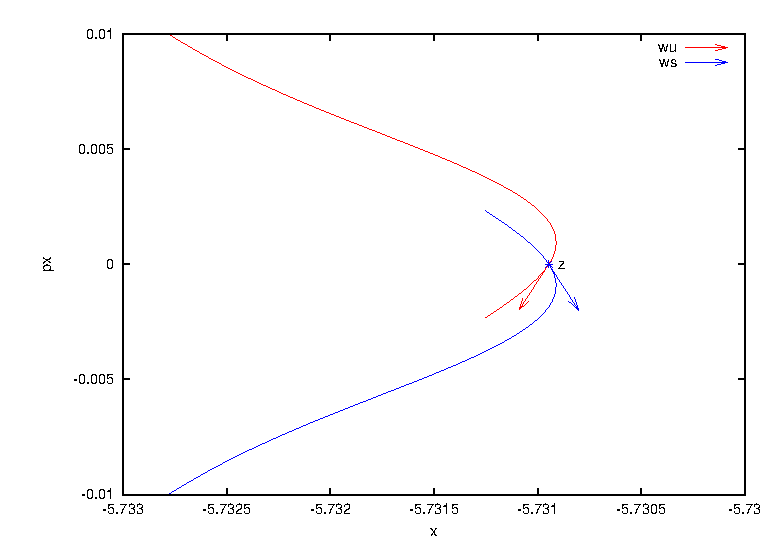
\includegraphics{figs/splitangle}
\caption{Outer splitting of the manifolds for energy level $H=-1.74$. 
This is a magnification of Figure~\ref{fig:invmfld2_it23_H174} at the
intersection point~$z_1$. 
We show the vectors $w_u, w_s$ tangent to the unstable and stable
manifolds at $z_1$. 
The splitting angle $\sigma$ is the angle between $w_u$ and $w_s$.}
\label{fig:splitangle}
\end{figure}

Due to reversibility, the vector $w_s$ tangent to the stable manifold
at $z_1$
is $w_s=(w_1,-w_2)$. See Figure~\ref{fig:splitangle}. Notice that we
choose the tangent vectors with the appropriate orientation, i.e. with
the same orientation as the trajectories on the manifolds. 

Thus the oriented splitting angle between $w_u$ and $w_s$ is 
\[ \sigma= 2\arctan_2(-w_1,-w_2), \]
where $\arctan_2$ is the arctangent function of two variables, which
uses the signs of the two arguments to determine the sign of the
result.

\begin{figure}
\psfrag{H}{$H$}
\psfrag{s}{$\sigma$ (radians)}
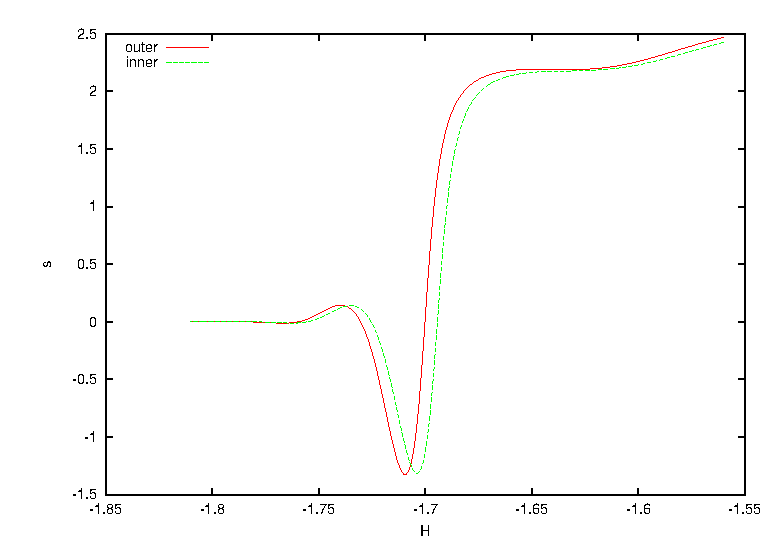
\includegraphics{figs/splittings}
\caption{Splitting angle associated to inner and outer splitting.}
\label{fig:splittings}
\end{figure}

\begin{table}
\begin{tabular}{|c|c|}
\hline
inner & outer \\
\hline
$ ( -1.695,-1.694 ) $ & $ ( -1.701,-1.700 ) $ \\
$ ( -1.726,-1.725 ) $ & $( -1.731,-1.730 ) $ \\
$ ( -1.756,-1.755 ) $ & $ ( -1.760,-1.759 ) $ \\
$ ( -1.781,-1.780 ) $ & $ ( -1.784,-1.783 ) $ \\
$ ( -1.802,-1.801 ) $ & $ ( -1.805,-1.804 ) $ \\
\hline
\end{tabular}
\caption{Subintervals of $H\in[H_-,H_+]$ containing the zeros of inner
splitting (left column) and outer splitting (right column).}
\label{tab:zeros_inner_outer}
\end{table}



Finally, we let $H$ change and, using this procedure, we are able to
obtain the splitting angle for energy levels $H \in [H_-, H_+]$.
See Figure~\ref{fig:splittings}.
The splitting angle is nonzero for all energy values except for a
discrete set of them.  
The splitting angle oscillates around zero with decreasing amplitude
as $H\to H_-$.
Numerically, we find that the zeros of the splitting angle are
contained in the intervals listed in
Table~\ref{tab:zeros_inner_outer}.

Notice that the inner and outer splittings behave similarly.
%See Figure~\ref{fig:splittings}.
However, they become zero at different values of $H$, as seen in
Table~\ref{tab:zeros_inner_outer}.
Thus, when one of the intersections becomes tangent, the other one is
still transversal, and we can always use one of them for diffusion. 


\subsection{Accuracy of the Computations}
\label{sec:accuracy_computations}

For small eccentricities, the splitting angle~$\sigma$ becomes very
small.
We need to check the validity of $\sigma$, making sure that the size
of (accumulated) numerical errors in the computation is smaller than
the size of $\sigma$.

The smallest splitting angle in Figure~\ref{fig:splittings},
corresponding to $H_-=-1.81$, is
\[ \sigma(H_-)= -1.777970294158603 \times 10^{-5}. \]
We check the validity of $\sigma(H_-)$ by recomputing this angle using
an alternative numerical method.
First we compute the intersection of the manifolds $W^{u,1}(p_3)$ and
$W^{s,1}(p_2)$ with the horizontal axis defined by
\[ p_x = \frac{j}{10^{5}} \]
for $j\in (-2,-1,1,2)$.

\begin{table}
\begin{tabular}{|c|c|c|c|}
\hline
$p_x$ & $x^u$ & $x^s$ & $x^u-x^s$ \\
\hline
$-0.00002$ & $-5.481541931871417$ & $-5.481541932226887$ &
$0.000000000355470$ \\
$-0.00001$ & $-5.481541931790012$ & $-5.481541931967703$ &
$0.000000000177691$ \\
$0.00000$ & $-5.481541931822124$ & $-5.481541931822124$ &
$0.000000000000000$ \\
$0.00001$ & $-5.481541931967703$ & $-5.481541931790012$ &
$-0.000000000177691$ \\
$0.00002$ & $-5.481541932226887$ & $-5.481541931871417$ &
$-0.000000000355470$\\
\hline
\end{tabular}
\caption{Sampling of the manifolds $W^{u,1}(p_3)$ and $W^{s,1}(p_2)$ at
different values of $p_x$, and their difference (last column).}
\label{tab:differentiation}
\end{table}

In Table~\ref{tab:differentiation} we tabulate the $x$ coordinate of
$W^{u,1}(p_3)$ and $W^{s,1}(p_2)$ on these axis, and their difference
$d=x^u-x^s$ gives the distance between the manifolds.
We apply numerical differentiation to the last column of this table,
using central differences centered at $z_1$ with step sizes $0.00002$
and $0.00004$, and obtain the values:
\[ d_1 = \frac{d(0.00001) - d(-0.00001)}{0.00002} =
-0.0000177691.\]
\[ d_2 = \frac{d(0.00002) - d(-0.00002)}{0.00004} =
-0.0000177735.\]
Finally, we use Richardson extrapolation and obtain:
\[ d = \frac{4 d_1-d_2}{3} = -0.00001776763333333333. \]
Thus, using this alternative method, we obtain the splitting angle
\[ \sigma(H_-) = \mathrm{atan}(-0.00001776763333333333) =
-0.00001776763333146364. \]
Compare the splitting angle computed using the two methods. They
differ by approximately $10^{-8}$.
This gives an estimate of the numerical error commited in our
computation of the splitting angle.

\begin{figure}
\psfrag{H}{$H$}
\psfrag{srad}{$\sigma$ (radians)}
\psfrag{s}{$\sigma$}
\psfrag{err}{$\mathrm{err}$}
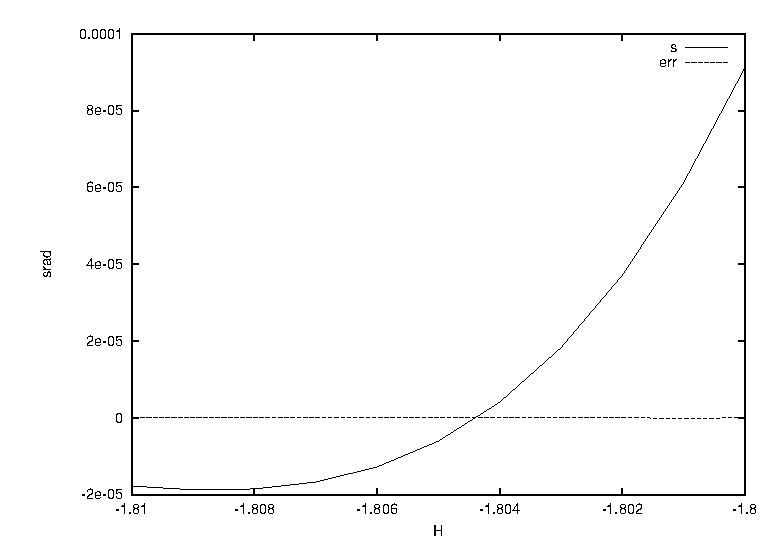
\includegraphics{figs/diffs}
\caption{Splitting angle $\sigma(H)$ and estimate of the numerical
error $\mathrm{err}(H)$ as a function of energy level $H$.}
\label{fig:diffs}
\end{figure}

We repeat this test for a range of energies $H\in[-1.81,-1.8]$.
In Figure~\ref{fig:diffs}, we compare the splitting angle $\sigma(H)$
and the estimate of the numerical error $\mathrm{err}(H)$. This error stays
below $10^{-7}$, and it is several orders of magnitude smaller than
the splitting angle.
For higher energy values $H\in[-1.8,-1.56]$, the splitting angle is
large, so the numerical error is certainly smaller.
Therefore we are confident that the splitting angle has been accurately
computed in the range of eccentricities considered,
$[H_-,H_+]$.


\section{Geometric structure of the resonance in Delaunay coordinates}
\label{sec:geometric_structure_delaunay}

Explain that the Poincar\'e sections in Cartesian and Delaunay are very
different. Explain that, after we transform periodic points to
Delaunay, we have to flow them a little forward or backwards until
they lie on the {g=0} section.

Show a picture of the resonance (periodic points, inv. manifolds) in
Delaunay.

\section{Numerical study of the inner and outer dynamics}
\label{sec:NumericalStudyInnerOuter}

\subsection{Inner and outer dynamics of the circular problem}
\label{app:InnerOuterCircular}

In this section, we numerically compute the inner map $\FF_0^\inn$ and
the outer maps $\FF_0^{\out,\ast}$ of the circular problem, given in
Section~\ref{Section:Circular}.
XXX Change of notation: $H$ instead of $I$. XXX

As seen in Section~\ref{sec:Circular:Inner}, the inner map has the
form
\begin{equation}\label{def:InnerMap:Circular:Numerics}
  \FF_0^\inn:\left(\begin{array}{c} H\\
      t
    \end{array}\right)\mapsto \left(\begin{array}{c} H\\
      t+\mu\TTT_0(H)
    \end{array}\right),
\end{equation}
where $T_H = 14\pi + \mu\TTT_0(H)$ is the period of the periodic orbit
obtained in Theorem~\ref{th:NHIMCircular} on the corresponding energy
surface.

Recall that we computed the periodic orbit $\gamma_H$ as well as its
period $T_H$ in Section~\ref{sec:computation_periodic_orbits}.
In particular, Figure~\ref{fig:porbits} shows a plot of the function
$T_H - 14\pi = \mu\TTT_0(H)$. 
Notice that the derivative of the function $\TTT_0(H)$ is nonzero for
the whole range $[\bar H_-, \bar H_+]$ of energy values. 
This shows that the inner map is twist. 
Moreover, Figure~\ref{fig:porbits} shows that 
\[ 0<\mu\TTT_0(H)<60\mu<\pi. \]
Therefore, the function $\TTT_0(H)$ satisfies the properties
stated in Lemma~\ref{lem:TwistInner}

As a test, we have computed the same function $\TTT_0(H)$ using two
different methods. First by computing the period of the periodic
orbit, as above. Then by computing the integral
expression~\eqref{def:T0:Integral} using numerical integration. The
difference in $\TTT_0(H)$ using both methods is of the order
$10^{-12}$.

As seen in Section~\ref{sec:Circular:Outer}, the outer maps have the
form
\begin{equation}\label{def:OuterMap:Circular:Numerics}
  \FF_0^{\out,\ast}:\left(\begin{array}{c} H\\
      t
    \end{array}\right)\mapsto \left(\begin{array}{c} H\\
      t+\mu\omega^\ast(H)
    \end{array}\right),\,\,\,\ast=\ff,\bb.
\end{equation}
For simplicity, let us only discuss the computation of $\omega^\ff(H)$
($\omega^\bb(H)$ is computed analogously).
Recall from Lemma~\ref{lem:Omega0} that the function $\omega^\ff(H)$
is defined as
  \[
  \omega^\ff(H)= \omega^\ff_\out(H)+\omega_\inn^\ff (H),
  \]
where, taking into account that the homoclinic orbit is symmetric with respect to the involution \eqref{def:involution},
\begin{equation}\label{def:Omega0:OuterPart:Numerics}
 \omega^\ff_\out(H)=\omega_+^\ff(H)-\omega^\ff_-(H) = 2\omega_+^\ff(H)
\end{equation}
  with
  \begin{equation}\label{def:Omega0PlusMinus:Numerics}
 \begin{split}  
 \omega_+^\ff(H)&=\lim_{N\rightarrow+\infty}\left(\int_0^{ 14N\pi
      }\frac{(\pa_G\Delta
        H_\ccirc) \circ \gamma_H^\ff(\sigma)}{-1+\mu(\pa_G\Delta
        H_\ccirc) \circ \gamma_H^\ff(\sigma)} \,
d\sigma+N\TTT_0(H)\right),\,\,\,
\end{split}  
\end{equation}
\begin{equation}\label{def:Omega0:InnerPart:Numerics}
\begin{split}
 \omega_\inn^\ff(H)&=\int_0^{ -12\pi
      }\frac{(\pa_G\Delta
        H_\ccirc) \circ \gamma_H^4(\sigma)}{-1+\mu(\pa_G\Delta
        H_\ccirc) \circ \gamma_H^4(\sigma)} \, d\sigma.
\end{split}
\end{equation}
To obtain $\omega^\ff(H)$, we compute the
integrals~\eqref{def:Omega0PlusMinus:Numerics}
and~\eqref{def:Omega0:InnerPart:Numerics} numerically, using a standard
algorithm from the GSL library XXX Add reference XXX.
The integrals are computed within a relative error limit $10^{-9}$.

The function $\pa_G\Delta H_\ccirc$ involved in both integrals is
given explicitly in Appendix~\ref{sec:RotatingToDelaunay}.
The integral $\omega_\inn^\ff(H)$ is evaluated on a periodic
trajectory $\gamma_H^4(\sigma)$ of the circular problem with initial
condition $p_4$, a fixed point of the Poincar\'e map $\PP_0^7$
found in Section~\ref{sec:geometric_structure_delaunay}.
The integral $\omega_+^\ff(H)$ is evaluated on a homoclinic trajectory
$\gamma_H^\ff(\sigma)$ of the circular problem with initial condition
$z_2$, the primary homoclinic point corresponding to the inner
splitting found in Section~\ref{sec:homoclinic_points}.

Next we make a couple of important remarks about the numerical
computation of the integral $\omega_+^\ff(H)$.
The key point is that the homoclinic orbit $\gamma_H^\ff$ was already
computed in section~\ref{sec:homoclinic_points} with high accuracy,
and we can exploit this information here.
Recall that the primary homoclinic point $z_2$ was obtained as the
$n$-th iterate of a point $z_u$ in the local fundamental segment $l_u$
under the Poincar\'e map:
\begin{equation} \label{eq:zu_to_z2}
 z_2 = \{\PP_0^7\}^n (z_u).
\end{equation}
Moreover, recall that the point $z_u$ was chosen to be suitably close
to the fixed point $p_3$ for each energy level $H$.
See Remark~\ref{rem:displacement}. 

Notice that the integral $\omega_+^\ff(H)$ is defined by a limit as
$N\to\infty$, i.e. as the homoclinic orbit $\gamma_H^\ff(\sigma)$
assymptotically approaches the periodic orbit $\gamma_H^3(\sigma)$ in
forward time (see equation~\eqref{def:OmegaSmall}).
Numerically, of course, we should stop integrating at an upper
endpoint $N$ large enough such that the integral converges. 
In practice, we choose the upper endpoint $N=N(H)$ to be the number of
iterates $n=n(H)$ in~\eqref{eq:zu_to_z2}.
This means that we evaluate the integral along the homoclinic
trajectory $\gamma_H^\ff(\sigma)$ until it reaches the point $z_u$,
which is suitably close to the periodic orbit.

Notice also that integrating the homoclinic trajectory
$\gamma_H^\ff(\sigma)$ forwards in the reduced system means
integrating it backwards along the unstable manifold in the original
system. 
This is numerically unstable, since numerical errors grow
exponentially. 
In practice, we rewrite the
integral~\eqref{def:Omega0PlusMinus:Numerics} using the change of
variables $\hat \sigma = \sigma - 14N\pi$ so that the homoclinic
trajectory is integrated forwards along the unstable manifold,
starting from the point $z_u$.

\begin{figure}
\psfrag{H}{$H$}
\psfrag{wf}{$\omega^{\ff}$}
\psfrag{wb}{$\omega^{\bb}$}
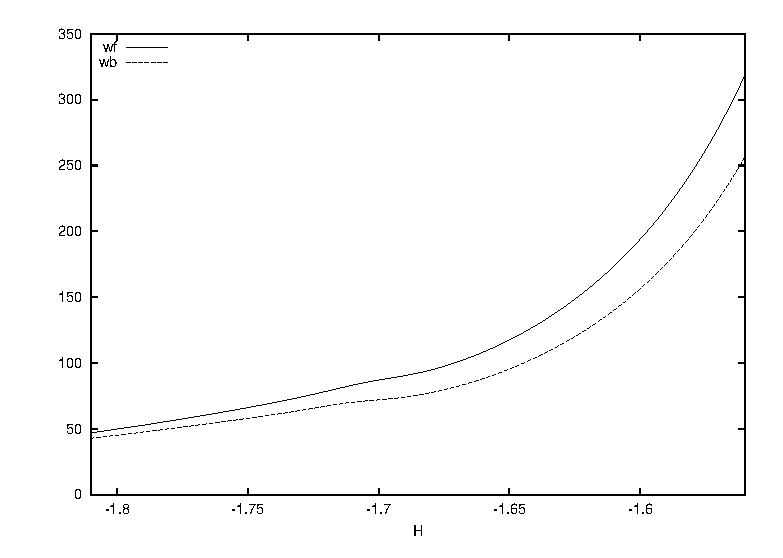
\includegraphics{figs/omega_fb}
\caption{Functions $\omega^{\ff}$ and $\omega^{\bb}$ involved in the
definition of the outer map~\eqref{def:OuterMap:Circular:Numerics} of
the circular problem.}
\label{fig:outer_circular}
\end{figure}

The computed values of the functions $\omega^{\ff}$ and $\omega^{\bb}$
are shown in Figure~\ref{fig:outer_circular}.

To test the computation of the function $\omega_+^\ff$, we directly
verify the definition of the outer map~\ref{definition:OuterMap}.
Let $z_2 = (L_h,\ell_h,G_h,0)$ be the primary homoclinic point, and
let $p_3 = (L_p,\ell_p,G_p,0)$ be the periodic point. 
Given a point $(L_h,\ell_h,G_h,0, I, t)$ in the extended circular
problem, we check that it is forward assymptotic (in the
reparametrized time) to the point $(L_p,\ell_p,G_p,0, I,
t+\omega_+^\ff)$, where $t\in\TT$ is arbitrary.
Thus we check that the distance
\[ \mathrm{dist}^+(s) = |\Phi_0\{s,(L_h,\ell_h,G_h,0, I, t)\} - 
\Phi_0\{s,(L_p,\ell_p,G_p,0, I, t+\omega_+^\ff)\}| 
\xrightarrow{s\to\infty} 0 \]
with exponential decay.

\begin{figure}
\psfrag{N}{$N$}
\psfrag{d}{$dist^+$}
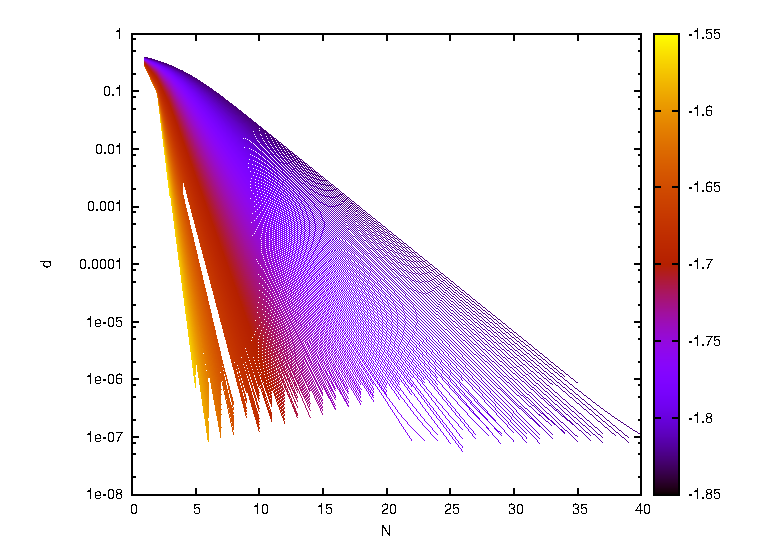
\includegraphics{figs/outer_circ_test}
\caption{Exponential decay of the function $\mathrm{dist}^+$ as a function of
$N$ (multiples of the period) for different energy levels.
The energy levels $H\in[H_-,H_+]$ are color-coded.}
\label{fig:outer_circ_test}
\end{figure}

The result of the test is shown in Figure~\ref{fig:outer_circ_test}
for values of the energy $H\in[H_-,H_+]$.  
Notice that the vertical axis is in logarithmic scale. 
Let $s=14N\pi$. 
We plot the distance $\mathrm{dist}^+$ as a function of $N$ (multiples of the
period). 
The test shows exponential decay of the distance function for all
energy values, i.e. straight lines in the plot. 

Recall that the periodic orbit $\gamma_H$ becomes more hyperbolic as
the energy $H$ increases. Thus, the rate of exponential convergence
between the homoclinic and the periodic trajectory also increases,
i.e. the straight lines have increasing slope in the plot.
As explained above, the length of integration $N=N(H)$ along the
homoclinic orbit is suitably chosen for each energy level.
For energy values $H\to H_-$, there is exponential decay up to
time $s=40\cdot (14\pi) \approx 1760$.



\subsection{Inner and outer dynamics of the elliptic problem}
\label{app:InnerOuterElliptic}

In this section, we numerically compute the first orders in $e_0$ of
the inner map $\FF_{e_0}^\inn$ and the outer maps
$\FF_{e_0}^{\out,\ast}$ of the elliptic problem, given in
Section~\ref{sec:Elliptic}. 
In order to compare the inner and outer dynamics of the elliptic
problem through Lemma~\ref{lemma:Averaging}, only some specific terms
in the expansions of the inner and outer maps are necessary. 
Namely, we only need to compute the term $A_1$ in the expansion of the
inner map~\eqref{def:InnerMap:ell}, and the term $B^*$ in the
expansion of the outer map~\eqref{def:OuterMap:Elliptic}.

Recall from section~\ref{sec:CylinderExpansion} that $A_1$ can be
split as 
  \[
  A_1(I,t)=A_1^+(I)e^{it}+A_1^-(I)e^{-it}.
  \]
Since $A_1^+$ and $A_1^-$ are complex conjugate, it is only necessary
to compute one of them. Let us compute the positive harmonic,
  \begin{equation}\label{def:A:plus:Numerics}
    A_1^+(I)=-i\mu\int_0^{-14\pi}\frac{\Delta H_{\eell}^{1,+}\circ
\gamma_I^3(\sigma)}{-1+\mu\pa_G\Delta
H_\ccirc\gamma_I^3(\sigma)}e^{i\wt\gamma_I^3(\sigma)}d\sigma.
  \end{equation}
Notice that the denominator is the same one used in the previous
section for the inner and outer dynamics of the circular problem. 
Next we give the numerator $i\Delta H_{\eell}^{1,+}$ explicitly.
Let 
  \begin{equation}\label{def:Ham:Elliptic:order1}
    \begin{split}
      \Delta H^1_\eell(L,\ell,G,g,t) =&
-\frac{1-\mu}{\mu}\BB_1\left(-\frac{r(L,\ell,G)}{\mu},v(L,\ell,G),g,t\right)\\
      &-\frac{\mu}{1-\mu}\BB_1\left(\frac{r(L,\ell,G)}{1-\mu},v(L,\ell,G),g,t\right),
    \end{split}
  \end{equation}
  where $\BB_1$ is the function defined in Lemma
\ref{lemma:ExpansionB}.
%%%%%%%%%%%%%%%%%%%%%%%%%%%%%
\begin{comment}
We write $B_1$ as a sum of harmonics 
\begin{align*}
B_1(r,v+g,t) 
   &= B_1^+(r,v+g)e^{it}+B_1^-(r,v+g)e^{-it} \\
   &=-\frac{1-r\cos(v+g)-i2r\sin(v+g)}{2\Delta^3(r,v+g)}e^{it}
-\frac{1-r\cos(v+g)+i2r\sin(v+g)}{2\Delta^3(r,v+g)}e^{-it}.
\end{align*}
Thus we have
\[ B_1^+(r,v+g) =
-\frac{1-r\cos(v+g)-i2r\sin(v+g)}{2\Delta^3(r,v+g)}. \]

Writing $\Delta H_{\eell}^1$ as a sum of harmonics, we have
\begin{equation}
  \begin{split}
\Delta H_{\eell}^{1,+} =&
-\frac{1-\mu}{\mu}\BB_1^+\left(-\frac{r(L,\ell,G)}{\mu},v(L,\ell,G),g,t\right)\\
      &-\frac{\mu}{1-\mu}\BB_1^+\left(\frac{r(L,\ell,G)}{1-\mu},v(L,\ell,G),g,t\right).
  \end{split}
\end{equation}
\end{comment}
%%%%%%%%%%%%%%%%%%%%%%%%%%%%%
Then it is straightforward to see that 
\begin{equation}
  \begin{split}
\Delta H_{\eell}^{1,+}(l,L,g,G)
=& 
-\frac{1-\mu}{\mu}\BB_1^+\left(-\frac{r(L,\ell,G)}{\mu},v(L,\ell,G),g\right)
\\
      &-\frac{\mu}{1-\mu}\BB_1^+\left(\frac{r(L,\ell,G)}{1-\mu},v(L,\ell,G),g\right),
  \end{split}
\end{equation}
where
\[ \BB_1^+(r,v,g) =
-\frac{1-r\cos(v+g)-i2r\sin(v+g)}{2\Delta^3(r,v+g)}. \]

\begin{figure}
\psfrag{H}{$\hat H$}
\psfrag{A}{$A_1^+(I)$}
\psfrag{reXXXXXX}{$\Re(A_1^+)$}
\psfrag{imXXXXXX}{$\Im(A_1^+)$}
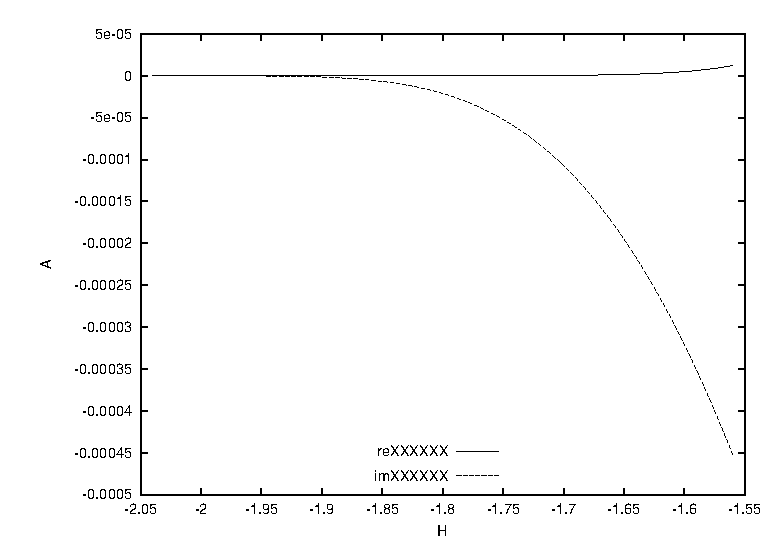
\includegraphics{figs/inner_ell}
\caption{Function $A_1^+(I)$ (real and imaginary parts) involved in
the definition of the inner map~\eqref{def:InnerMap:ell} of the
elliptic problem as a function of the energy of the system in rotating
coordinates $\hat H$. Recall that $\hat H = -I$.}
\label{fig:inner_ell}
\end{figure}

The computed value of the function $A_1^+$ is shown in
Figure~\ref{fig:inner_ell}.

For the outer map, we compute the functions $B^*(I)$.
Similarly to $A_1$, it is only necessary to compute the positive
harmonics $B^{*,+}$.
Recall from Lemma~\ref{lemma:Outer:Elliptic} that the positive
harmonics $B^{\ff,+}(I)$ and $B^{\bb,+}(I)$ are defined as 
\begin{equation}\label{def:Omega:PlusMinus:Numerics}
\begin{split}
B^{\ff,+}(I)&=B_\out^{\ff,+}(I)+B_\inn^{\ff,+}(I)e^{i\mu\omega_\out^\ff(I)}\\
B^{\bb,+}(I)&=B_\inn^{\bb,+}(I)+B_\out^{\bb,+}(I)e^{i\mu\omega_\inn^\bb(I)},
\end{split}
\end{equation}
where $\omega_\out^\ff$ and $\omega_\inn^\bb$ were obtained in
Section~\ref{app:InnerOuterCircular}.
To obtain $B_\out^{*,+}$ and $B_\inn^{*,+}$, we compute the
integrals~\eqref{def:Omega:PlusMinus:Out:for}--\eqref{def:Omega:PlusMinus:Inn}
numerically, using the same techniques as in the previous
section~\ref{app:InnerOuterCircular}.

\begin{figure}
\psfrag{H}{$\hat H$}
\psfrag{reBfXXXXXX}{$\Re(B^{\ff,+})$}
\psfrag{imBfXXXXXX}{$\Im(B^{\ff,+})$}
\psfrag{reBbXXXXXX}{$\Re(B^{\bb,+})$}
\psfrag{imBbXXXXXX}{$\Im(B^{\bb,+})$}
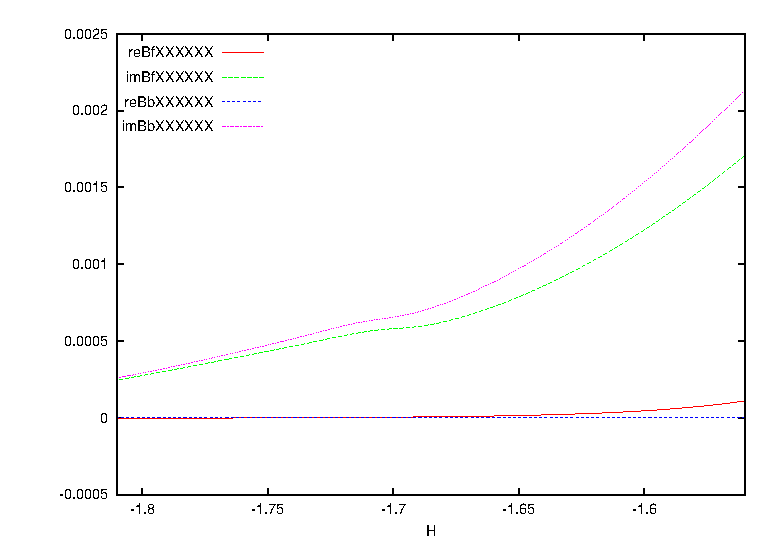
\includegraphics{figs/B_fb}
\caption{Functions $B^{\ff,+}$ and $B^{\bb,+}$ (real and imaginary parts) 
involved in the definition of the outer
map~\eqref{def:OuterMap:Elliptic} of the elliptic problem.}
\label{fig:B_fb}
\end{figure}

The computed values of the functions $B^{\ff,+}(I)$ and $B^{\bb,+}(I)$ are
shown in Figure~\ref{fig:B_fb}.


\subsection{Comparison of the inner and outer dynamics of the elliptic problem}\label{app:Comparison}

Finally, we verify the non-degeneracy
condition
 \begin{equation}\label{eq:NonVanishing:Outer:Numerics}
   \wt B^{\ast,\pm} \left(\II\right)\neq 0\qquad\text{for }\II\in
\DD^\ast
 \end{equation}
stated in Lemma~\ref{lemma:Averaging}, which implies the existence of
a transition chain of tori.
Since $B^{\ast,+}$ and $B^{\ast,-}$ are complex-conjugate, it is only
necessary to compute one of them. Let us compute the positive
harmonic,
 \[
 \wt B^{\ast,+} \left(\II\right)=B^{\ast,+}
\left(\II\right)-\frac{e^{i\mu\omega^\ast(\II)}-1}{e^{
i\mu\TTT_0(\II)}-1}A_1^+ \left(\II\right).
 \]
All the functions involved in the expression above are known: $\TTT_0$
and $\omega^\ast$ are obtained in
section~\ref{app:InnerOuterCircular}, $A_1^+$ and $B^{\ast,+}$ are
obtained in section~\ref{app:InnerOuterElliptic}.

\begin{figure}
\psfrag{H}{$\hat H$}
\psfrag{reBfXXXXXX}{$\Re(\wt B^{\ff,+})$}
\psfrag{imBfXXXXXX}{$\Im(\wt B^{\ff,+})$}
\psfrag{reBbXXXXXX}{$\Re(\wt B^{\bb,+})$}
\psfrag{imBbXXXXXX}{$\Im(\wt B^{\bb,+})$}
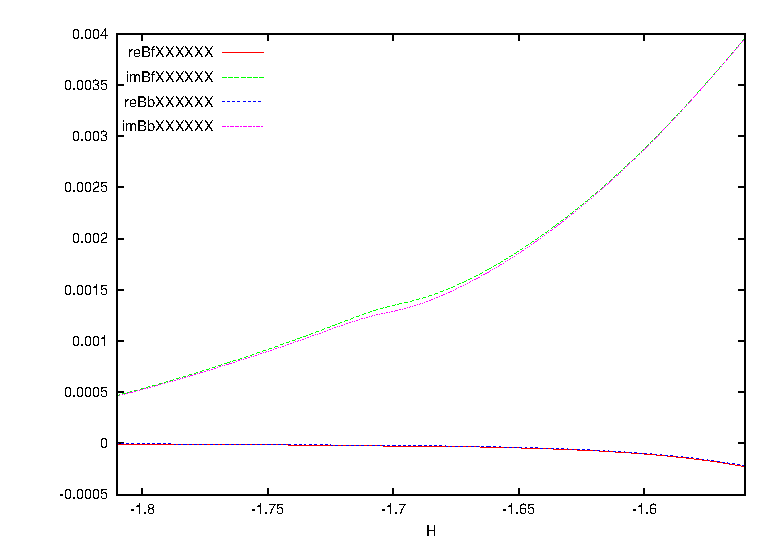
\includegraphics{figs/tildeB}
\caption{Functions $\wt B^{\ff,+}$ and $\wt B^{\bb,+}$ (real and
imaginary parts).}
\label{fig:tildeB}
\end{figure}

The computed values of the functions $\wt B^{\ff,+}$ and $\wt
B^{\bb,+}$ are shown in Figure~\ref{fig:tildeB}.
Therefore, we see that the functions $\wt B^{\ast,+}$ are not
identically zero.
This justifies the statement~\eqref{eq:NonVanishing:Outer} in
Lemma~\ref{lemma:Averaging}.

\begin{remark}
Figure~\ref{fig:tildeB} also shows that $\wt B^{\ff,+}$ and $\wt
B^{\bb,+}$ are almost identical, which is surprising for the authors.
However, this fact is not relevant for the argument in
Lemma~\ref{lemma:Averaging}; we only need that these functions do not
vanish identically.
\end{remark}
